
\section{Results}
% https://latexdraw.com/bar-charts-in-latex-step-by-step-tikz-tutorial/

\begin{frame}{LoDoPaB-CT dataset}
  \begin{itemize}
      \item Dataset for low-dose Computed Tomography
      \item 35'820 train samples
      \item 3'553 test samples
      \item BM3D as baseline algorithm
      \item Resolution 64 x 64
  \end{itemize}
  \begin{figure}
    \centering
    \hfill
    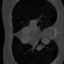
\includegraphics[width=0.16\textwidth]{ct_im_0.png}
    \hfill
    
\includegraphics[width=0.16\textwidth]{ct_im_1.png}
    \hfill
    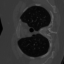
\includegraphics[width=0.16\textwidth]{ct_im_2.png}
    \hfill
    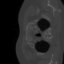
\includegraphics[width=0.16\textwidth]{ct_im_3.png}
    \hfill
    \caption{Some samples from the LoDoPaB-CT dataset.}
  \end{figure}
\end{frame}


\begin{frame}{GAT-Denoiser - Implementation for Computed Tomography}
  \begin{itemize}
    \item PyTorch Geometric
    \item U-Net used for reconstruction
    \begin{itemize}
        \item Pre-trained with complete dataset and $SNR_y$ in [-10, 0] dB for 200 epochs
        \item Joint U-Net training possible
    \end{itemize}
    \item Mini-batch gradient descent with batch size 64
    \item Adam optimizer
    
  \end{itemize}
\end{frame}




\begin{frame}{Evaluation}
\begin{itemize}
    \item Small Scale Experiments
    \begin{itemize}
        \item 1024 train samples
        \item 100 test samples
        \item 200 epochs
        \item<2> \alert{Goal: Find most promising architecture}
    \end{itemize}
    \item Large Scale Experiments
    \begin{itemize}
        \item Complete LoDoPaB-CT dataset
        \item 20 - 40 epochs
        \item<2> \alert{Goal: Find best model}
    \end{itemize}
\end{itemize}
\end{frame}

\begin{frame}{Small Scale Experiments - Overall Results}
    \begin{columns}
        \column{0.52\textwidth}
        \begin{itemize}
            \item Learning fails with random graph (Erdős–Rényi)
            \item Learning succeeds with defined input graph
            \item<2-> Single components contribute to success of GAT-Denoiser:
            \begin{itemize}
              \item \alert{GAT: 2 layers and 4 heads}
              \item \alert{Convolution: kernel size 3 and padding 1}
              \item \alert{k-NN with k=2}
              \item \alert{Joint U-Net training}
            \end{itemize}
        \end{itemize}
        \column{0.47\textwidth}
        \begin{figure}
          \centering
          \begin{subfigure}[t]{0.4\textwidth}
              
\includegraphics[width=\textwidth]{random__graph_small_experiment.png}
              \caption{Reconstruction with random Erdős–Rényi graph with $p=0.01$}
          \end{subfigure}\hfill
          \begin{subfigure}[t]{0.4\textwidth}
              
\includegraphics[width=\textwidth]{knn__graph_small_experiment.png}
              \caption{Reconstruction with k-NN input graph $k = 10$}
          \end{subfigure}
      \end{figure}
        
    \end{columns}
\end{frame}

\begin{frame}{Large Scale Experiment - SNR Results}
  \only<1>{
    \begin{itemize}
      \item 3'553 test samples
      \item Different algortihms / GAT-Denoiser models:
      \begin{itemize}
        \item FBP
        \item BM3D
        \item GAT + U-Net (10/30)
        \item Conv + GAT + U-Net (20/20)
      \end{itemize}
      \item Reconstruction SNR averages over all test samples
    \end{itemize}
  }
    \only<2>{
      \begin{figure}
        \centering
        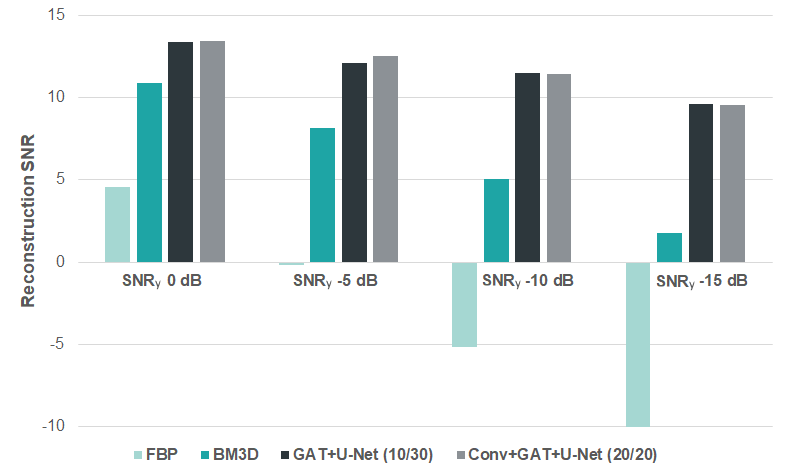
\includegraphics[width=.7\textwidth]{LargeScaleResults.png}
    \end{figure}
    }
    
\end{frame}

\begin{frame}{Large Scale Experiment - Visual Results - $SNR_y$ 0 dB}
\begin{figure}
    \captionsetup[subfigure]{justification=centering}
    \centering
    \begin{subfigure}[t]{0.18\textwidth}
      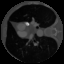
\includegraphics[width=\textwidth]{clean/clean_6.png}
      \caption{Clean sample}
    \end{subfigure} \hfill
    \begin{subfigure}[t]{0.18\textwidth}
      
\includegraphics[width=\textwidth]{fbp/0/fbp_0_6.png}
      \caption{FBP}
    \end{subfigure} \hfill
    \begin{subfigure}[t]{0.18\textwidth}
      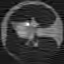
\includegraphics[width=\textwidth]{bm3d_reco/0/bm3d_reco_0_6.png}
      \caption{BM3D}
    \end{subfigure} \hfill
    \begin{subfigure}[t]{0.18\textwidth}
      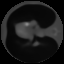
\includegraphics[width=\textwidth]{gat_unet/0/gat_unet_0_6.png}
      \caption{\textit{GAT+U-Net(10/30)}}
    \end{subfigure} \hfill
    \begin{subfigure}[t]{0.18\textwidth}
      
\includegraphics[width=\textwidth]{conv_gat_unet/0/conv_gat_unet_0_6.png}
      \caption{\textit{Conv+GAT+U-Net(20/20)}}
    \end{subfigure} \hfill
    \caption{Large Scale Experiment: Visual results for $SNR_y$ 0 dB.}
  \end{figure}
  

  \begin{tcolorbox}[colback=red!5!white,hide=<1>, alert=<2>, colframe=red!75!black]
    GAT-Denoiser improves BM3D for $SNR_y$ 0 dB  by 27.6\%.
    \end{tcolorbox}
    
\end{frame}


\begin{frame}{Large Scale Experiment - Visual Results - $SNR_y$ -10 dB}
    \begin{figure}
        \captionsetup[subfigure]{justification=centering}
        \centering
        \begin{subfigure}[t]{0.18\textwidth}
          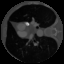
\includegraphics[width=\textwidth]{clean/clean_6.png}
          \caption{Clean sample}
        \end{subfigure} \hfill
        \begin{subfigure}[t]{0.18\textwidth}
          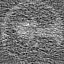
\includegraphics[width=\textwidth]{fbp/-10/fbp_-10_6.png}
          \caption{FBP}
        \end{subfigure} \hfill
        \begin{subfigure}[t]{0.18\textwidth}
          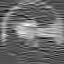
\includegraphics[width=\textwidth]{bm3d_reco/-10/bm3d_reco_-10_6.png}
          \caption{BM3D}
        \end{subfigure} \hfill
        \begin{subfigure}[t]{0.18\textwidth}
          
\includegraphics[width=\textwidth]{gat_unet/-10/gat_unet_-10_6.png}
          \caption{\textit{GAT+U-Net(10/30)}}
        \end{subfigure} \hfill
        \begin{subfigure}[t]{0.18\textwidth}
          
\includegraphics[width=\textwidth]{conv_gat_unet/-10/conv_gat_unet_-10_6.png}
          \caption{\textit{Conv+GAT+U-Net(20/20)}}
        \end{subfigure} \hfill
        \caption{Large Scale Experiment: Visual results for $SNR_y$ -10 dB.}
      \end{figure}
      
    
      \begin{tcolorbox}[colback=red!5!white,hide=<1>, alert=<2>, colframe=red!75!black]
        GAT-Denoiser improves BM3D for $SNR_y$ -10 dB by 126.0\%.
        \end{tcolorbox}
        
\end{frame}

\begin{frame}{Large Scale Experiment - Visual Results - $SNR_y$ -15 dB}
    \begin{figure}
        \captionsetup[subfigure]{justification=centering}
        \centering
        \begin{subfigure}[t]{0.18\textwidth}
          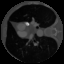
\includegraphics[width=\textwidth]{clean/clean_6.png}
          \caption{Clean sample}
        \end{subfigure} \hfill
        \begin{subfigure}[t]{0.18\textwidth}
          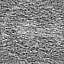
\includegraphics[width=\textwidth]{fbp/-15/fbp_-15_6.png}
          \caption{FBP}
        \end{subfigure} \hfill
        \begin{subfigure}[t]{0.18\textwidth}
          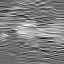
\includegraphics[width=\textwidth]{bm3d_reco/-15/bm3d_reco_-15_6.png}
          \caption{BM3D}
        \end{subfigure} \hfill
        \begin{subfigure}[t]{0.18\textwidth}
          
\includegraphics[width=\textwidth]{gat_unet/-15/gat_unet_-15_6.png}
          \caption{\textit{GAT+U-Net(10/30)}}
        \end{subfigure} \hfill
        \begin{subfigure}[t]{0.18\textwidth}
          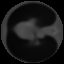
\includegraphics[width=\textwidth]{conv_gat_unet/-15/conv_gat_unet_-15_6.png}
          \caption{\textit{Conv+GAT+U-Net(20/20)}}
        \end{subfigure} \hfill
        \caption{Large Scale Experiment: Visual results for $SNR_y$ -15 dB.}
      \end{figure}
      
    
      \begin{tcolorbox}[colback=red!5!white,hide=<1>, alert=<2>, colframe=red!75!black]
        GAT-Denoiser improves BM3D for $SNR_y$ -15 dB by 379.9\%.
        \end{tcolorbox}
        
\end{frame}
